% vim:et:sw=2:ts=2:enc=iso-8859-15:fenc=iso-8859-15

\mode<presentation> {
  \usetheme{RWTHRZ}
}

\usepackage[german]{babel}
\usepackage[latin1]{inputenc}
\usepackage{times}
\usepackage[T1]{fontenc}
\usepackage[right]{eurosym}
\usepackage{graphicx}
\usepackage{hyperref}
\usepackage{color}
\definecolor{red}{rgb}{0.9,0.2,0.2}
\definecolor{green}{rgb}{0.2,0.5,0.2}
\definecolor{blue}{rgb}{0.2,0.2,0.5}
\definecolor{darkblue}{rgb}{0,0,.5}
\definecolor{lightgray}{rgb}{0.9,0.9,0.9}
\definecolor{gray}{rgb}{0.4,0.4,0.4}
\hypersetup{pdftex=true, colorlinks=true, breaklinks=true, linkcolor=darkblue, menucolor=darkblue, pagecolor=darkblue, urlcolor=darkblue}

\title[Einf�hrung in Ruby on Rails]{Einf�hrung in Ruby on Rails}
\author[Gilger, Lederhofer]{}
\date[\today]{\today}

\begin{document}

\begin{frame}
  \begin{center}
    \vspace*{\fill}
    \Huge Einf�hrung in Ruby on Rails \\
    \vspace{0.8cm}
    
\includegraphics[scale=2]{img/ruby-logo.png} \enskip
    
\includegraphics[scale=0.6]{img/rails-logo.png} \\
    \vspace{0.6cm}
    \Large Johannes Gilger \& Matthias Lederhofer \\
    \small Rechen- und Kommunikationszentrum der RWTH Aachen \\
    \vspace{1cm}
    \small \today
    \vspace*{\fill}
  \end{center}
\end{frame}

\begin{frame}
  \frametitle{�bersicht}
  \begin{itemize}
    \item Ruby
    \item Rails
    \item Warum man Rails benutzen m�chte
    \item Konzepte (DRY, MVC, Convention over Configuration)
    \item ActiveRecord - ORM
    \item Weiterf�hrende Literatur
  \end{itemize}
\end{frame}


\begin{frame}
  \frametitle{Der Name}
  \begin{center}
    \Huge Ruby \pause on Rails
  \end{center}
\end{frame}

\begin{frame}
  \frametitle{Der Name}
  \begin{center}
    \Huge {\color{red}Ruby} on Rails
  \end{center}
\end{frame}

\begin{frame}
  \frametitle{Ruby}
  \begin{itemize}
    \item Objektorientierte, interpretierte Sprache
    \item Dynamisch getyped
    \item Sehr einfache Syntax
  \end{itemize}
\end{frame}

\begin{frame}
  \frametitle{Ruby: Klassen}
  { \tt \small
  class Customer \\
  \enskip attr\_accessor :vorname, :nachname \\
  \enskip \\
  \enskip def initialize \\
  \enskip \enskip @vorname = @nachname = '''' \\
  \enskip end \\
  \enskip \\
  \enskip def name \\
  \enskip \enskip return @vorname + '' '' + @nachname \\
  \enskip end \\
  end \\
  }
  \begin{center}
    \small Keine Getter/Setter-Methoden schreiben:
  \end{center}
  { \tt \small
  jojo = Customer.new \\
  jojo.vorname = ''Johannes'' \\
  }
\end{frame}

\begin{frame}
  \frametitle{Ruby: Datentypen}
  { \tt \small [0, 1, 2, ''hallo'', 23.5] } - Array \\
  { \tt \small \%w(Jan, Feb, Mar, Apr)} - Stringarray \\
  { \tt \small \{ ''jojo'' => 24, ''matled'' => 25 \}} - Hash \\
  \vspace{0.3cm}
  \begin{center}
    \emph{Alle} Datentypen sind Objekte und besitzen ein Vielzahl praktischer Methoden
  \end{center}
\end{frame}

\begin{frame}
  \frametitle{Ruby: Beispiele}
  {\tt \small 2.times \{puts ''Hello''\}} \\
  {\tt \small {\color{green}=> 'Hello'}} \\
  {\tt \small {\color{green}=> 'Hello'}}
  \vspace{0.5cm}
  \pause

  {\tt \small ''RWTH Aachen''.downcase.split('''').uniq.sort.join} \\
  {\tt \small  {\color{green}=> '' acehnrtw''}} \\
  \vspace{0.5cm}
  \pause

  {\tt \small array = [1, 'hi', 3.14]} \\
  {\tt \small array.each \{|item| puts item\}} \\
  {\tt \small {\color{green}=> 1}} \\
  {\tt \small {\color{green}=> 'hi'}} \\
  {\tt \small {\color{green}=> 3.14}}
  \vspace{0.5cm}
  \pause

  {\tt \small (1..10).collect \{|x| x*x\}} \\
  {\tt \small {\color{green}=> [1, 4, 9, 16, 25, 36, 49, 64, 81, 100]}}
\end{frame}

\begin{frame}
  \frametitle{Der Name}
  \begin{center}
    \Huge Ruby {\color{red}on Rails}
  \end{center}
\end{frame}

\begin{frame}
  \frametitle{Rails}
  \begin{itemize}
    \item{Open-Source Web-Applikation Framework auf Grundlage von Ruby}
    \item{Aufgeteilt in mehrere Komponenten}
    \begin{itemize}
      \item{ActiveRecord - ORM (Datenbankanbindung)}
      \item{ActiveResource, ActionPack, ActiveSupport, ActionMailer}
    \end{itemize}
    \vspace{0.3cm}

    \item{2004: Ver�ffentlichung, seitdem viele Ver�nderungen}
    \item{2008: Rails-Entwicklung wird von SVN auf git umgestellt}
    \item{2010: Rails 2.3.5 ist stable, Rails l�uft auch auf Ruby 1.9}
    \vspace{0.3cm}

    \item{Bekannte Projekte unter Rails:}
    \begin{itemize}
      \item{GitHub, Twitter, Lighthouse, XING, etc.}
    \end{itemize}
  \end{itemize}
\end{frame}

\begin{frame}
  \frametitle{Warum man Rails benutzen m�chte}
  \begin{itemize}
    \item{Sehr schnelle Entwicklung von Webanwendungen \\ Insbesondere das initiale Interface}
    \item{Unabh�ngigkeit von Datenbank-Engine durch Abstraktion \\ Dadurch auch ein Sicherheitsvorteil}
    \item{Vermeidung von h�ufig wiederholten und eigentlich einfachen Operationen}
    \item{Vereinbarung bestimmter Konventionen die das Zusammenarbeiten einfacher machen}
    \item{Hilfreiche Werkzeuge zum Entwickeln und Debuggen}
  \end{itemize}
\end{frame}

\begin{frame}
  \frametitle{Convention over Configuration}
  Rails trifft bestimmte Annahmen:
  \vspace{0.5cm}
  \begin{itemize}
    \item Datenbank: Tabellen sind pluralisiert (Person => people). Jede Tabelle hat einen Prim�rschl�ssel ''id'' (INT)
    \item Datenbank: Fremschl�ssel heissen person\_id
    \item Applikation: Aufteilung in MVC und Ordner
  \end{itemize}
  \vspace{0.5cm}
  Resultat: Einschr�nkungen die befreien. Grundlegende Entwicklungst�tigkeiten werden sehr einfach.
\end{frame}

\begin{frame}
  \frametitle{MVC - Model, View, Controller}
  \begin{center}
    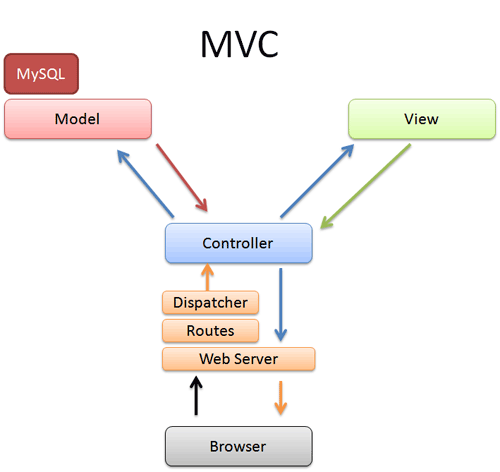
\includegraphics[width=7.5cm]{img/mvc.png}
  \end{center}
\end{frame}

\begin{frame}
  \frametitle{MVC - Model, View, Controller}
  \begin{center}
    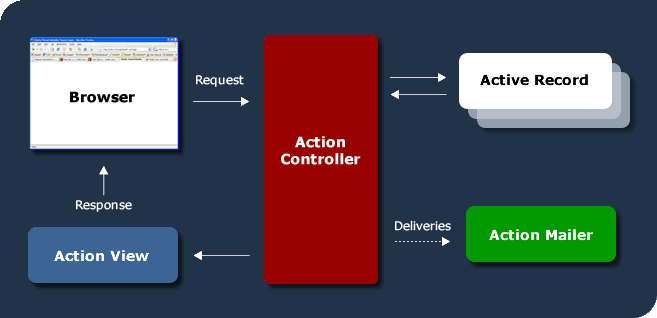
\includegraphics[width=9.5cm]{img/mvc_rails.png}
  \end{center}
\end{frame}

\begin{frame}
  \frametitle{ORM - Object Relational Mapper}
  {\tt \small CREATE TABLE people (''vorname'' VARCHAR(255),} \\
  {\tt \small \enskip ''nachname'' VARCHAR(255));} \\
  \vspace{0.3cm}
  \pause

  {\tt \small class Customer < ActiveRecord::Base} \\
  {\tt \small \enskip def name} \\
  {\tt \small \enskip \enskip return self.vorname + '' '' + self.nachname} \\
  {\tt \small \enskip end} \\
  {\tt \small end} \\
  \vspace{0.3cm}
  \pause

  {\tt \small jojo = Customer.create(:vorname => ''Johannes'',} \\
  {\tt \small \enskip :nachname => ''Gilger'')} \\
  \vspace{0.3cm}
  \pause

  {\tt \small puts jojo.name} \\
  {\tt \small {\color{green}=> ''Johannes Gilger''}}
\end{frame}

\begin{frame}
  \frametitle{DRY - Don't Repeat Yourself}
  {\tt \small CREATE TABLE customers (''vorname'' VARCHAR(255),} \\
  {\tt \small \enskip ''nachname'' VARCHAR(255));} \\
  \vspace{0.3cm}

  {\tt \small class Customer < ActiveRecord::Base} \\
  {\tt \small \enskip def name} \\
  {\tt \small \enskip \enskip return self.vorname + '' '' + self.nachname} \\
  {\tt \small \enskip end} \\
  {\tt \small end} \\
  \vspace{0.3cm}
  \pause

  \begin{center}
  Wo kommen Customer.vorname und Customer.nachname her? \\
  \pause
  \vspace{0.1cm}
  => {\tt Customer} ist Unterklasse von {\tt ActiveRecord::Base}! \\
  \vspace{0.3cm}
  \end{center}
  Klasse: Tabelle ({\tt class Customer}) \\
  Instanz: Zeile einer Tabelle ({\tt jojo = Customer.new}) \\
  Attribut einer Instanz: Zelle ({\tt jojo.vorname = ''Johanna''})
\end{frame}

\begin{frame}
  \frametitle{DRY - Models}
  Validation in den Models, alles was in die Datenbank soll wird �ber das Model geleitet \\
  \tt \small
  \vspace{0.5cm}
  class Customer < ActiveRecord::Base \\
  \enskip validates\_uniqueness\_of :login, :on => :create \\
  \enskip validates\_confirmation\_of :password \\
  \enskip validates\_length\_of :login, :within => 3..40 \\
  \enskip validates\_length\_of :password, :within => 5..40 \\
  end
\end{frame}

\begin{frame}
  \frametitle{ActiveRecord - Assoziationen}
  Assoziationen machen Arbeiten mit zusammenh�ngenden Daten sehr einfach \\
  \tt \small
  \vspace{0.5cm}
  class Order < ActiveRecord::Base \\
  \enskip belongs\_to :customer \\
  end \\
  \vspace{0.3cm}
  class Customer < ActiveRecord::Base \\
  \enskip has\_many :orders \\
  end \\
  \vspace{0.5cm}
  ich = Customer.find\_by\_vorname(''Johannes'') \\
  ich.orders \\
  {\color{green}=> [\#order1, \#order2, \ldots]}
\end{frame}

\begin{frame}
  \frametitle{ActiveRecord - Assoziationen}
  \begin{center}
    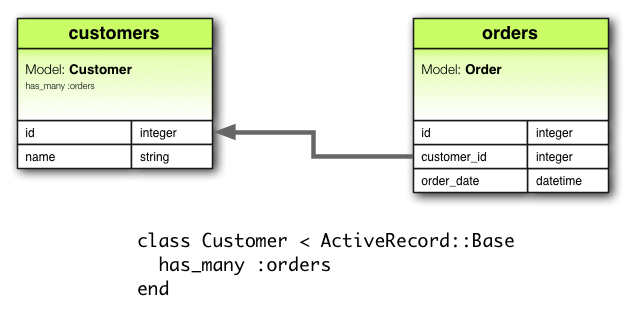
\includegraphics[width=10.5cm]{img/has_many.png}
  \end{center}
\end{frame}

\begin{frame}
  \frametitle{ActiveRecord - Assoziationen}
  \begin{center}
    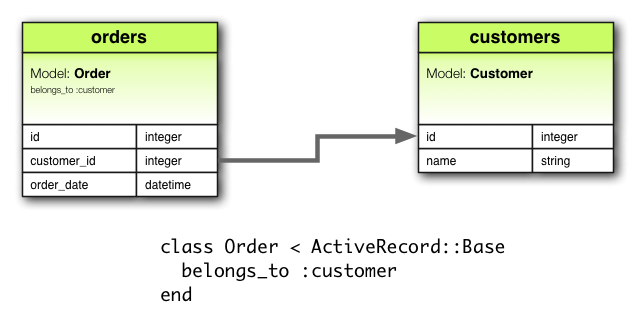
\includegraphics[width=10.5cm]{img/belongs_to.png}
  \end{center}
\end{frame}

\begin{frame}
  \frametitle{ActiveRecord - Assoziationen}
  \begin{center}
    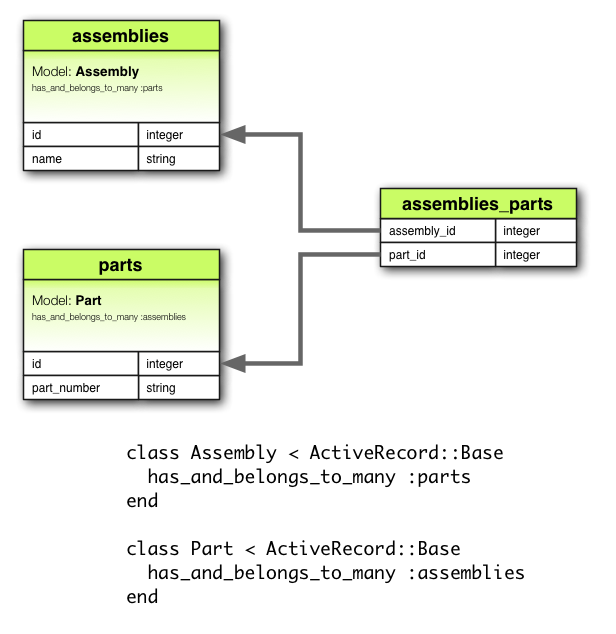
\includegraphics[width=7.5cm]{img/habtm.png}
  \end{center}
\end{frame}

\begin{frame}
  \frametitle{Der Controller}
  Die Aufgaben des Controllers kann man unterteilen in
  \begin{enumerate}
    \item Daten aus einem oder mehreren Models holen (sprich: Instanzen)
    \item Eventuell etwas mit diesen Daten machen
    \item Daten an ein View weitergeben zur Anzeige
  \end{enumerate}
\end{frame}

\begin{frame}
  \frametitle{Controller \& View}
  {\bf \small app/controllers/people\_controller.rb}\\
  { \tt \small
    class {\color{red}People}Controller < ApplicationController \\
    \enskip def {\color{green}list} \\
    \enskip \enskip @customers = Customer.find :all \\
    \enskip end \\
    end \\
  }
  \vspace{0.3cm}
  {\small \bf app/views/people/list.rhtml} \\
  { \tt \small
    <table> \\
    \enskip <\% @customers.each do customer \%> \\
    \enskip \enskip <tr><td><\%= customer.vorname \%></td> \\
    \enskip \enskip \enskip <td><\%= customer.nachname \%></td></tr> \\
    \enskip <\% end \%> \\
    </table>
  }
  \begin{center}
    Aufruf von {\tt http://localhost:3000/{\color{red}people}/{\color{green}list}}
  \end{center}
\end{frame}

\begin{frame}
  \frametitle{Trennung Controller \& View}
  Aufgaben: \\
  \begin{itemize}
    \item {\bf Controller}: Programmlogik
    \item {\bf View}: Darstellung / Layout
  \end{itemize}

  Aufbau: \\
  \begin{itemize}
    \item {\bf Controller}: Einfach Ruby-Klasse
    \item {\bf View}: eRuby, Embedded Ruby in HTML (wie z.B. PHP)
  \end{itemize}
  Beispiel: \\
  \small \tt
  <\% 3.times do \%> \\
  \enskip <b><\%= ''Hello World'' \%></b><br/> \\
  <\% end \%>
\end{frame}

\begin{frame}
  \frametitle{Rails - Anwendungsordner}
  \begin{center}
    Neue Rails-Applikation mit: {\tt rails neuesprojekt}
    \pause
    \small \tt
    \begin{columns}[t]
      \begin{column}{5cm}
        app \\
        \enskip controllers \\
        \enskip helpers \\
        \enskip models \\
        \enskip views \\
        config \\
        db \\
        doc \\
        lib \\
        log \\
        public \\
        script \\
        test \\
        tmp \\
        vendor
      \end{column}
      \pause
      \begin{column}{5cm}
        app \\
        \enskip controllers \\
        \enskip helpers \\
        \enskip models \\
        \enskip views \\
        \pause
        config \\
        \pause
        {\color{gray}db} \\
        {\color{lightgray}doc} \\
        {\color{lightgray}lib} \\
        {\color{gray}log} \\
        public \\
        \pause
        script \\
        {\color{lightgray}test} \\
        {\color{lightgray}tmp} \\
        {\color{lightgray}vendor}
      \end{column}
    \end{columns}
  \end{center}
\end{frame}

\begin{frame}
  \frametitle{Rails - Anwendungsordner}
  \pause
  \small
  {\tt app} \\
  \enskip {\tt controllers} \\ \enskip\enskip Controller, verbinden Models und Views \\
  \enskip {\tt helpers} \\ \enskip\enskip Hilfsmethoden die in mehreren Controllern benutzt werden \\
  \enskip {\tt models} \\ \enskip\enskip Models (entsprechend z.B. den Tabellen in der Datenbank) \\
  \enskip {\tt views} \\ \enskip\enskip HTML-Templates die zur Anzeige der Webseite benutzt werden \\
  {\tt config} \\ \enskip\enskip Anwendungs- \& Datenbankkonfiguration \\
  {\tt public} \\ \enskip\enskip Statische �ffentliche Dateien (Bilder, Stylesheets) \\
  {\tt script} \\ \enskip\enskip Rails Hilfsprogramme und Debugging-Tools \\
\end{frame}

\begin{frame}
  \frametitle{Rails - Entwicklungshilfen}
  \pause
  \small
  {\tt script} \\
  \enskip {\tt console} \\ \enskip\enskip Ruby-Konsole, schnelles Testen von z.B. Models\\
  \enskip {\tt dbconsole} \\ \enskip\enskip Praktischer Shortcut, User/Passwort aus {\tt config/database.yml} \\
  \enskip {\tt generate} \\ \enskip\enskip Allround-Generator f�r Grundger�ste (Controllers, Models, etc.) \\
  \enskip {\tt plugin} \\ \enskip\enskip Plugins installieren \\
  \enskip {\tt server} \\ \enskip\enskip Entwicklungs-Webserver auf localhost:3000 starten
\end{frame}

\begin{frame}
  \frametitle{Rails - Installation \& Maintenance}
  Ruby benutzt eigene Paketverwaltung: \emph{RubyGems} \\
  \vspace{0.3cm}
  Vorteile:
  \begin{itemize}
    \item Schnelle und einfache Installation auch kleiner Programme
    \item Programme (''Gems'') sind unabh�ngig von Distribution
    \item Parallele Installation verschiedener Versionen
  \end{itemize}
  \vspace{0.3cm}
  Befehle:
  \begin{itemize}
    \item {\tt gem list $--$local} - Installierte Gems anzeigen
    \item {\tt gem install <name>} - Gem laden und installieren
    \item {\tt gem update} - Installierte Gems updaten
  \end{itemize}
\end{frame}

\begin{frame}
  \frametitle{Rails - Installation \& Maintenance}
  Rails benutzt Version mit der das Projekt erstellt wurde. Bei einem
  Update der Gems ({\tt rails, activerecord, ...}) wird \emph{nicht} automatisch
  die neuste Version benutzt. \\
  \vspace{0.3cm}
  Rails-Applikation updaten: \\
  \vspace{0.2cm}
  In {\tt config/environment.rb} muss {\tt RAILS\_GEM\_VERSION} angepasst werden.
\end{frame}

\begin{frame}
  \frametitle{Rails - Alternativen}
  Rails ist \emph{ein} Framework von vielen:
  \begin{itemize}
    \item {\bf Symfony} (PHP) \\ \url{http://www.symfony-project.org/}
    \item {\bf CakePHP} (PHP) \\ \url{http://cakephp.org/}
    \item {\bf Django} (Python) \\ \url{http://www.djangoproject.com/}
    \item {\bf Merb} (Ruby) \\ \url{http://www.merbivore.com/}
    \item {\bf Catalyst} (Perl) \\ \url{http://www.catalystframework.org/}
  \end{itemize}
  Viele neuere Frameworks verhalten sich wie Rails
\end{frame}

\begin{frame}
  \frametitle{Literatur zu Ruby \& Rails}
  \begin{itemize}
    \item {\bf Rails Guides} - \url{http://guides.rubyonrails.org/} \\ L�ngere Tutorials, generell und �ber einzelne Komponenten
    \item {\bf Agile Web Development with Rails, 3rd Edition} - The Pragmatic Bookshelf, ISBN: 978-1-93435-616-6 \\ Sehr ausf�hrliches Rails-Buch mit Tutorial-Teil
    \item {\bf Railscasts} - \url{http://railscasts.com/} \\ Kurze Screencasts zu einzelnen Techniken
    \item {\bf Ruby Class References} - \url{http://www.ruby-doc.org/docs/ProgrammingRuby/html/builtins.html} \\ Klassen- und Library-Referenz
    \item {\bf Rails API} - \url{http://api.rubyonrails.org/} \\ Rails API Dokumentation
  \end{itemize}
\end{frame}

\begin{frame}
  \frametitle{The End}
  \begin{center}
    \Huge Fragerunde!
    \vspace{1.5cm}

    \small Folgefragen k�nnen gerne an gilger@rz.rwth-aachen.de und lederhofer@rz.rwth-aachen.de gerichtet werden. \\
    Oder einfach vorbei schauen ;)
  \end{center}
\end{frame}

\end{document}
